\documentclass[a4paper, 12pt]{article}%тип документа

%Русский язык
\usepackage[T2A]{fontenc} %кодировка
\usepackage[utf8]{inputenc} %кодировка исходного кода
\usepackage[english,russian]{babel} %локализация и переносы

%отступы 
\usepackage[left=2cm,right=2cm,top=2cm,bottom=3cm,bindingoffset=0cm]{geometry}

%Вставка картинок
\usepackage{graphicx}
\graphicspath{}
\DeclareGraphicsExtensions{.pdf,.png,.jpg, .jpeg}

%Таблицы
\usepackage[table,xcdraw]{xcolor}
\usepackage{booktabs}
%Графики
\usepackage{pgfplots}
\pgfplotsset{compat=1.9}

%Математика
\usepackage{amsmath, amsfonts, amssymb, amsthm, mathtools}

%Заголовок
\author{Подлесный Артём \\ группа 827}
\title{ЗАДАЧА ТРЁХ ТЕЛ \\ Формулировка, современное состояние}

\begin{document}


\begin{figure}[h!]
\center{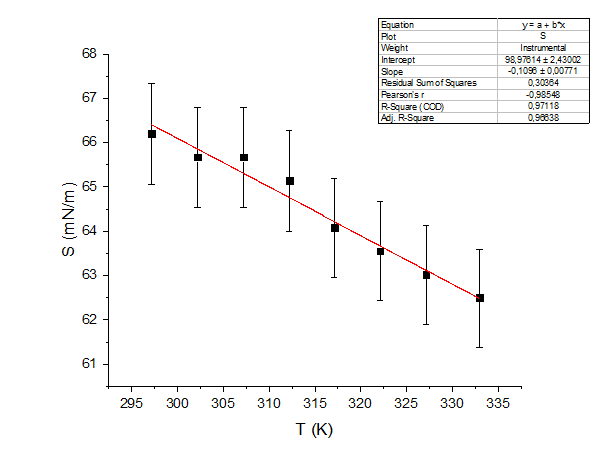
\includegraphics[scale=1.3]{gr1.png}}
\end{figure}

\begin{figure}[h!]
\center{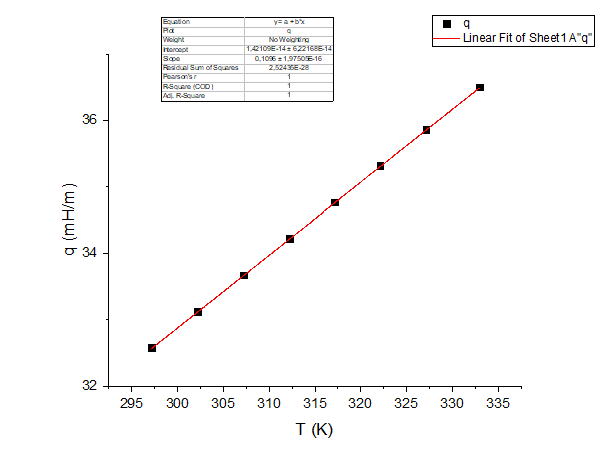
\includegraphics[scale=0.9]{gr2.png}}
\end{figure}

\begin{figure}[h!]
\center{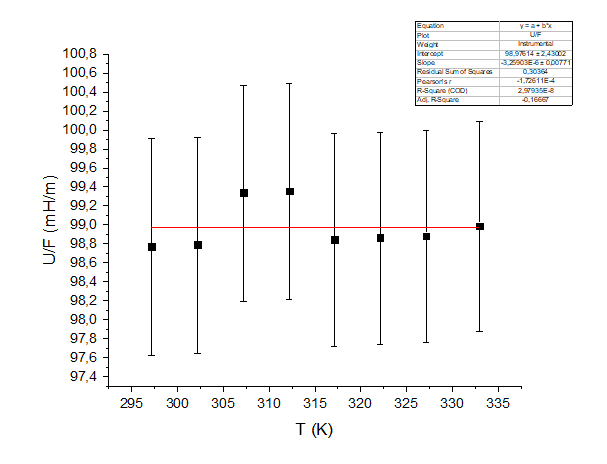
\includegraphics[scale=0.9]{gr4.png}}
\end{figure}


\end{document}